\documentclass[a4paper,11pt]{article}
\usepackage[utf8]{inputenc}
\usepackage{amsmath}
\usepackage{amsfonts}
\usepackage{amssymb}
\usepackage{graphicx}
\usepackage{braket}
\usepackage[font=small]{caption}

\numberwithin{equation}{section}
\renewcommand\thesubsection{\alph{subsection}}
\newcommand{\bvp}[1]{\mathbf{#1}'}
\newcommand{\bv}[1]{\mathbf{#1}}


%opening
\title{Computational Biophysics I HW1}
\author{Vince Baker}

\begin{document}

\maketitle

\section{Q1}
Biophysical simulations can be performed in any regime of temperature, volume, etc.
Theoretical results such as those of statistical mechanics are often only available for asymptotic systems (zero/infinite temperature, infinite volume). 
Computational biophysics extends the asymptotic theoretical results into arbitrary systems.\\
\\
Experimental biophysics requires substantial investment and can only collect certain types of data. 
Computational biophysics does not require specialized lab equipment and the entire experiment can be completely instrumented. 
Computational biophysics provides additional information not available in experiments and allows for inexpensive exploration of novel systems and concepts.
\section{Q2}
In a continuous potential very small differences in particle coordinates produce only small changes in the particle potential energy. 
For discrete potentials there are specific points at which a very small difference in position may produce a very large change in potential energy. 
Discontinuous potentials require the use of special techniques such as collision detection to correctly simulate motion near the discontinuities.
\section{Q3}
The force terms in the electrostatic and gravitational laws are both porportional to $r^2$. 
We take the field from a single proton as an example (mass $10^{-27}$, charge $10^{-19}$) with the appropriate constants of porportionality ($10^{-7}$ for electrostatic force, $10^{-11}$ for gravity).
So we see that the gravitational field strength is order $10^{-38}/r^2$ while the electrostatic field strength is order $10^{-26}/r^2$, a difference of $10^12$, so we are justified in ignoring the gravitational terms at atomic ranges.
\\
In most systems of interest the total net charge is approximately 0.
At longer length scales the electrostatic fields from the positive and negative charges will largely cancel, so that the attractive gravitational fields may become significant.
When the length scales are on the order of $10^{12}$ interatomic distances the gravitational field from the system will be of the same order as the electrostatic field from a single net charge.
\section{Q4}
Round-off errors are inherent in every digital simulation that represents continous variables. 
Round-off error can be reduced by using more bits to represent a quantity, but there will always be some error in the last bit and that error will grow with the number of operations performed.
\\
Truncation errors from numerical integration are also inevitable when integrating arbitrary continuous functions.
The error may be reduced by the choice of method and time step, but finite difference methods are inherently an approximation to he actual integral equation.
\section{Q5}
We express the fifth-order Gear predictor-corrector algorithm. 
We use the normal conventions for the first and second time derivatives $\bv{v}(t)$ and $\bv{a}(t)$ (velocity and acceleration).
The higher derivatives are written as $\bv{b}(t)$,$\bv{c}(t)$, etc..
The predicted system state at time $t+\delta t$ is given by the Taylor expansion of the state at time t:
\begin{align}
 \bv{r}(t+\delta t) &= \bv{r}(t)+\delta t \bv{v}(t) + \frac{1}{2}\delta t^2\bv{a}(t)+\frac{1}{6}\delta t^3\bv{b}(t)+\frac{1}{24}\delta t^4\bv{c}(t)+\frac{1}{120}\delta t^5\bv{d}(t)\\
 \bv{v}(t+\delta t) &= \bv{v}(t)+\delta t \bv{a}(t) + \frac{1}{2}\delta t^2\bv{b}(t)+\frac{1}{6}\delta t^3\bv{c}(t)+\frac{1}{24}\delta t^4\bv{d}(t)\\
 \bv{a}(t+\delta t) &= \bv{a}(t)+\delta t \bv{b}(t) + \frac{1}{2}\delta t^2\bv{c}(t)+\frac{1}{6}\delta t^3\bv{d}(t)\\
 \bv{b}(t+\delta t) &= \bv{b}(t)+\delta t \bv{c}(t) + \frac{1}{2}\delta t^2\bv{d}(t)\\
 \bv{c}(t+\delta t) &= \bv{c}(t)+\delta t \bv{d}(t)\\
 \bv{d}(t+\delta t) &= \bv{d}(t)
\end{align}
As in the third-order method, we calculate the acceleration at the predicted position. 
We can then calculate an error estimate for each term using the acceleration error $\Delta a(t+\delta t)=\bv{a}(t+\delta t)-\bv{a}(\bv{r}(t+\delta t))$.
The corrected system state is then expressed in terms of the acceleration error and experimentally determined coefficients.
\begin{align}
 \bv{r}_c(t+\delta t) &= \bv{r}(t+\delta t)+c_0 \Delta a(t+\delta t)\\
 \bv{v}_c(t+\delta t) &= \bv{v}(t+\delta t)+c_1 \Delta a(t+\delta t)\\
 \bv{a}_c(t+\delta t) &= \bv{a}(t+\delta t)+c_2 \Delta a(t+\delta t)\\
 \bv{b}_c(t+\delta t) &= \bv{b}(t+\delta t)+c_3 \Delta a(t+\delta t)\\
 \bv{c}_c(t+\delta t) &= \bv{c}(t+\delta t)+c_4 \Delta a(t+\delta t)\\
 \bv{d}_c(t+\delta t) &= \bv{d}(t+\delta t)+c_5 \Delta a(t+\delta t)
\end{align}

\section{Q6}
Writing the velocity Verlet algorithm and anpanding the expression for the velocity:
\begin{align}
 \bv{r}(t+\delta t) &= \bv{r}(t)+\delta t \bv{v}(t)+\frac{1}{2}\delta t^2 \bv{a}(t)\\
 \bv{r}(t+\delta t) &= \bv{r}(t)+\delta t \left\{\bv{v}(t-\delta t)+\frac{1}{2}\delta t\left(\bv{a}(t)+\bv{a}(t-\delta t) \right) \right\}+\frac{1}{2}\delta t^2 \bv{a}(t)\\
 \bv{r}(t+\delta t) &= \bv{r}(t)+\delta t \bv{v}(t-\delta t)+\delta t^2\bv{a}(t)+\frac{1}{2}\delta t^2\bv{a}(t-\delta t)
\end{align}
We now use the expression:
\begin{align}
 \bv{r}(t)-\bv{r}(t-\delta t) &= \delta t\bv{v}(t-\delta t)+\frac{1}{2}\delta t^2\bv{a}(t-\delta t)
\end{align}
Inserting into (3), we recover the Verlet expression for position:
\begin{align}
 \bv{r}(t+\delta t) &= 2\bv{r}(t)-\bv{r}(t)+\delta t^2\bv{a}(t)
\end{align}
This demonstrates that the Verlet and velocity Verlet methods will calculate the same trajectories.
\\
\section{Q7}
The ``Leapfrog'' method, in which the velocity and position are updated on staggered time steps, can be derived from the following Taylor expansions:
\begin{align}
 \bv{r}(t+\delta t) &= \bv{r}(t)+\delta t\bv{v}(t)+\delta t^2\frac{1}{2}\bv{a}(t)\\
 \bv{v}(t+\frac{1}{2}\delta t) &= \bv{v}(t)+\frac{1}{2}\delta t \bv{a}(t)\\
 \bv{v}(t-\frac{1}{2}\delta t) &= \bv{v}(t)-\frac{1}{2}\delta t \bv{a}(t)
\end{align}
From (1) and (2) we derive the position update equation:
\begin{align}
 \bv{r}(t+\delta t) &= \bv{r}(t)+\delta t\bv{v}(t+\frac{1}{2}\delta t)
\end{align}
From (2) and (3) we can derive the velocity update equation:
\begin{align}
 \bv{v}(t+\frac{1}{2}\delta t) &= \bv{v}(t-\frac{1}{2}\delta t)+\delta t\bv{a}(t)
\end{align}
Also, combining equations (2) and (3), we can derive an expression for $\bv{v}(t)$:
\begin{align}
 \bv{v}(t) &= \frac{1}{2}\left(\bv{v}(t+\frac{1}{2}\delta t)+\bv{v}(t-\frac{1}{2}\delta t) \right)
\end{align}

\section{Problem 1}
The standard deviation of the system energy is shown for the five timesteps in Figure 1. 
The slope of the linear fit line is 2.12, indicating that the Verlet integrator is a $O(\delta t^2)$ algorithm. 

\begin{figure}[h]
 \caption{Standard deviation of the system energy}
 \centering
   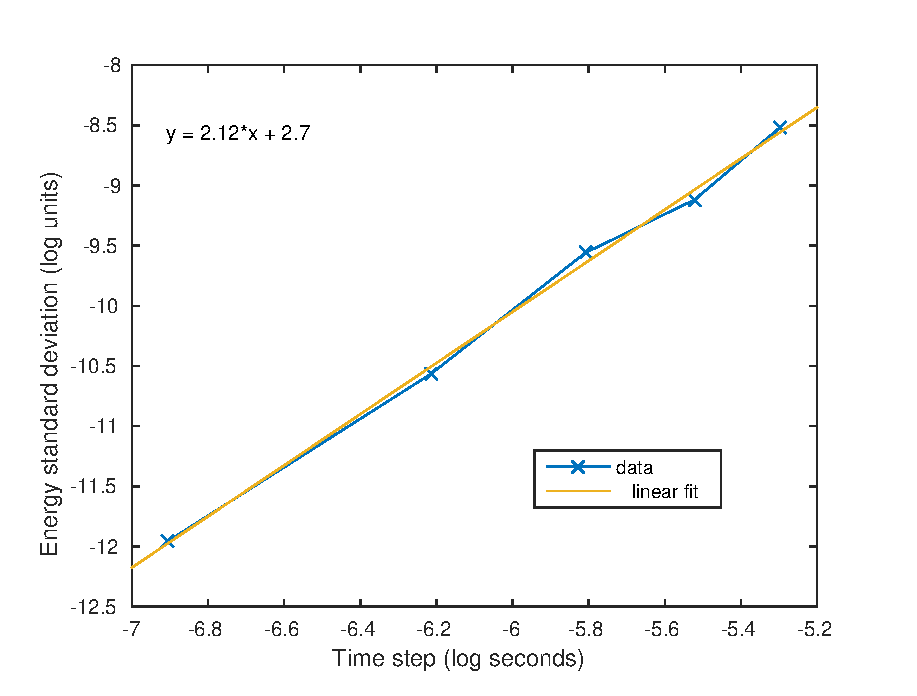
\includegraphics[width=0.5\textwidth]{EnergyStd}
 \label{fig:energystd}
\end{figure}

\begin{figure}[h]
 \caption{System energy over time}
 \centering
   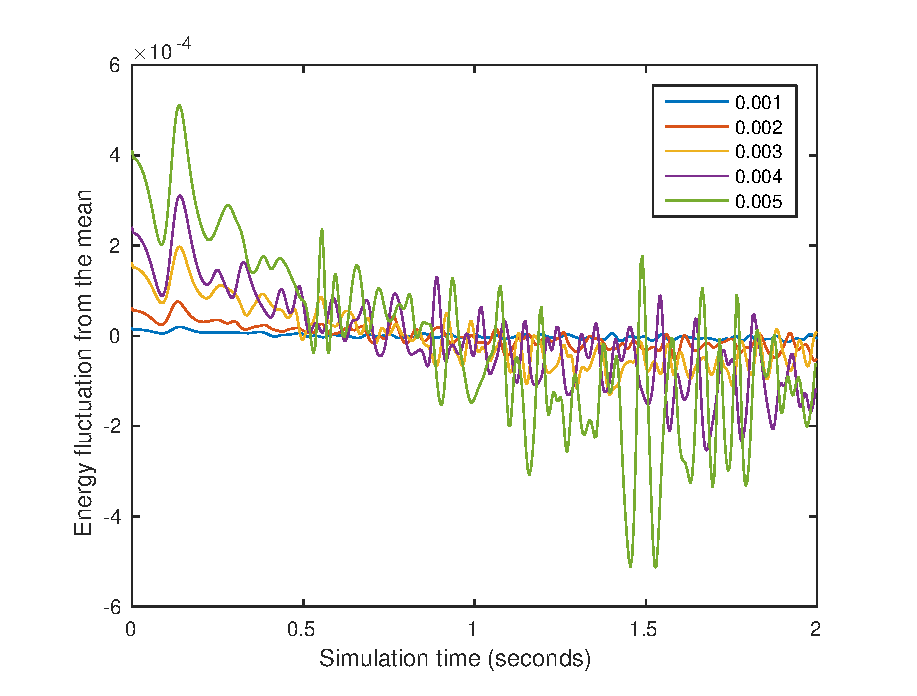
\includegraphics[width=0.5\textwidth]{EnergyPlot}
 \label{fig:energyplot}
\end{figure}

\end{document}
